\paragraph{}
in this section we will mention our final model and its performance.
we Have Three combinations we will illustrate.

\begin{enumerate}
	\item CNN .
	\item Hog and Landmarks .
	\item CNN with Hog and Landmarks .
\end{enumerate}
see Figure \ref{cnn_lm_hog} to check the model Architecture.
\begin{figure}
	\centering
	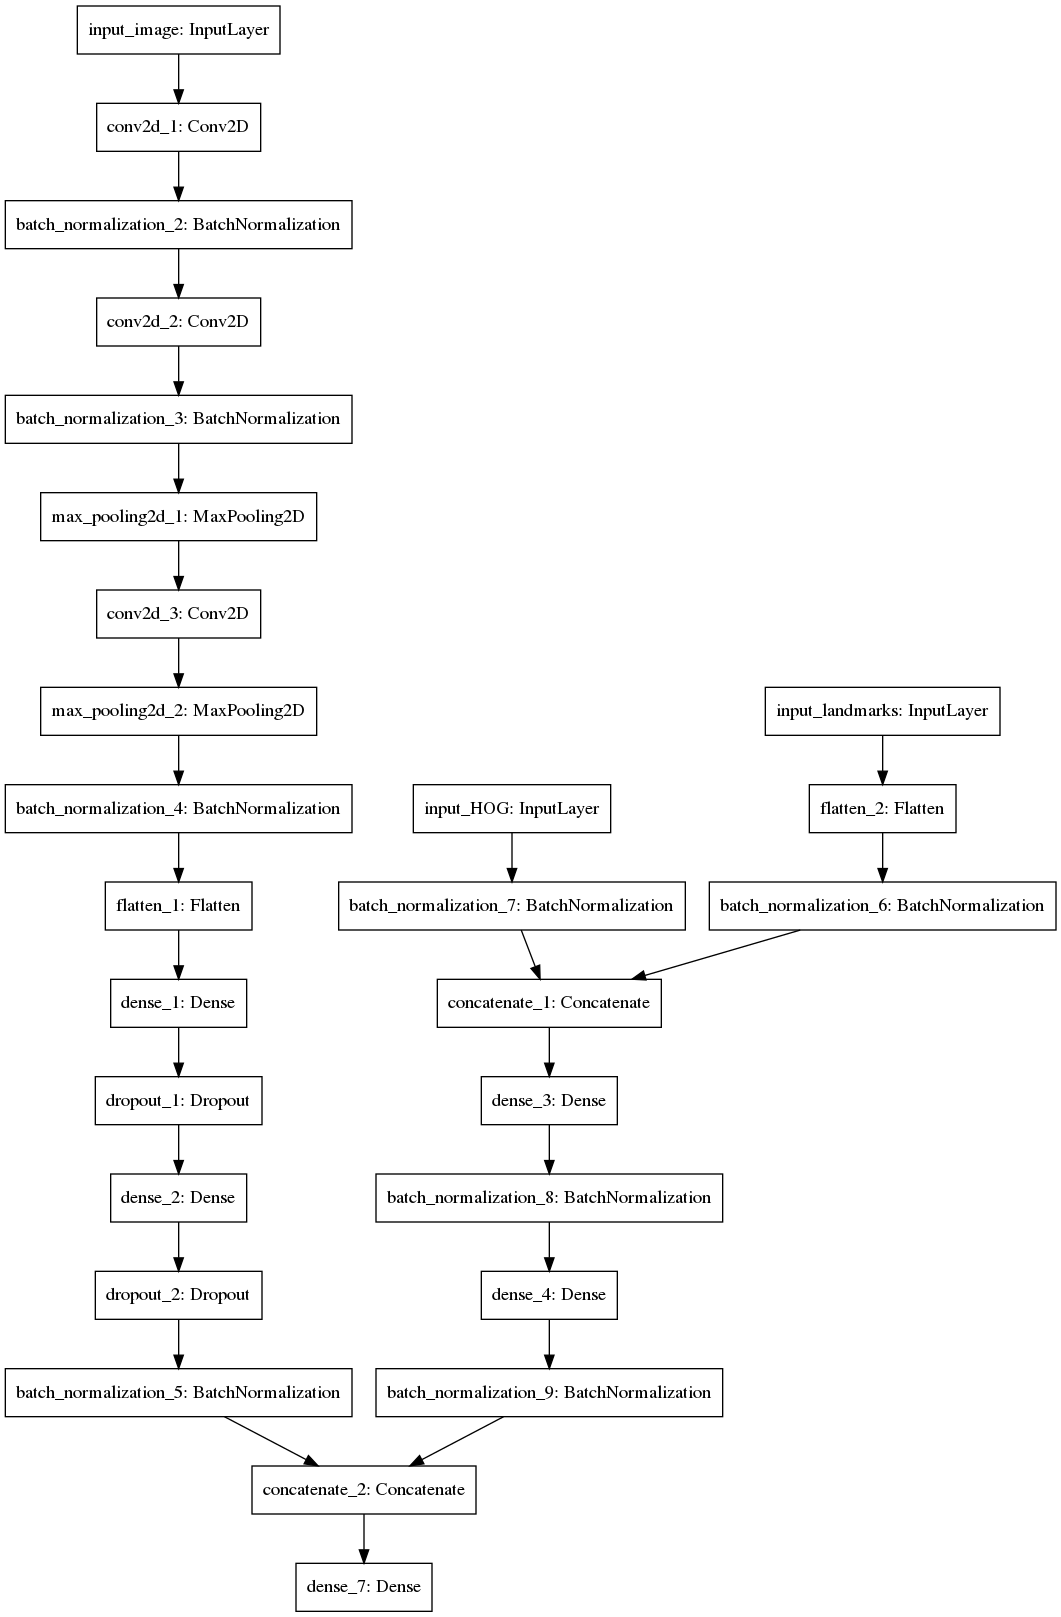
\includegraphics[width=1\textwidth]{images/cnn_hog_lm.png}
	\caption{Diagram of cnn+hog+lm structure}
	\label{cnn_lm_hog}
\end{figure}
\paragraph{}
We finally choose the model with only landmarks and hog path with final accuracy 98\% on the combination of ck+ and RafD dataset as the working model as we notice that :
\begin{enumerate}
	\item Using landmarks and hog as a feature extraction then feed it to model layers gives a good accuracy with small model size (1M) and the Training Process itself is too fast comparing with Cnn
	\item Using cnn model only works good give the same accuracy but the model size is large and take to much time in training .
	\item combine cnn with landmarks and hog , we do not notice any change in accuracy as cnn itself work as feature extraction so adding them together only make training process harder ,final model larger and no effect on the accuracy.
\end{enumerate} 